%!TEX root = ../main.tex
\section{Εισαγωγή στα FPGA}

Στο παρόν κεφάλαιο θα παραθέσουμε μερικές πληροφορίες σχετικά με το τι είναι ένα \gls{fpga}, την ιστορική εξέλιξή του και θα αναφερθούμε στις διάφορες εφαρμογές του στη βιομηχανία. Θα επιχειρήσουμε ακόμη μια σύντομη ανασκόπηση στις διάφορες καινοτομίες που έχουν συμβεί τα τελευταία χρόνια και βασίζονται στις ιδιαίτερα επιτυχημένες μονάδες FPGAs.

\subsection{Τι είναι το FPGA \& Σύντομη ιστορική αναδρομή}

Το \gls{fpga} είναι ένας τύπος προγραμματιζόμενου ολοκληρωμένου κυκλώματος σχεδιασμένο έτσι ώστε να διαμορφώνεται από τον πελάτη μετά την κατασκευή του, εξού και το όνομά του - field programmable. Η διαμόρφωση του γίνεται συνήθως με κάποια γλώσσα περιγραφής υλικού, παρόμοια με αυτές που χρησιμοποιούνται στα \gls{asic}.

Τα \gls{fpga} διαθέτουν έναν μεγάλο αριθμό τυποποιημένων προγραμματιζόμενων blocks και μια ιεραρχία από διαμορφώσιμες διασυνδέσεις που επιτρέπουν στα blocks να συνδέονται μεταξύ τους. Λογικά blocks μπορούν να διαμορφωθούν κατά τέτοιον τρόπο ώστε να πραγματοποιούν σύνθετες πράξεις ή απλές λογικές πύλες (AND, XOR, κά). Πολλά \gls{fpga} περιλαμβάνουν και διάφορες άλλες ψηφιακές λειτουργίες όπως απαριθμητές, καταχωρητές μνήμης, γεννήτριες PLL, DSP slices κα. Κατά τον προγραμματισμό του \gls{fpga} ενεργοποιούνται οι επιθυμητές λειτουργίες και διασυνδέονται μεταξύ τους έτσι ώστε το \gls{fpga} να συμπεριφέρεται ως ολοκληρωμένο κύκλωμα με συγκεκριμένη λειτουργία.

Η βιομηχανία των \gls{fpga} ξεκίνησε από την \gls{prom} και τις \glspl{pld}. Τόσο οι PROMs όσο και οι PLDs είχαν την επιλογή να προγραμματίζονται σε παρτίδες στο εργοστάσιο ή στο πεδίο. Η προγραμματιζόμενη λογική, ωστόσο, ήταν hard-wired μεταξύ των λογικών πυλών.

Η έννοια του \gls{fpga} αναπτύχθηκε στα τέλη της δεκαετίας του 1980 με την οικογένεια των XC2064TM \gls{fpga} της Xilinx. Την ίδια εποχή η Altera ανέπτυσσε τη δικιά της προγραμματιζόμενη συσκευή, την EP1200. Η τεχνολογία της Altera κατασκευαζόταν σε λιθογραφία 3-μm \gls{cmos} \gls{eprom} η οποία απαιτούσε υπεριώδη ακτινοβολία για να επαναπρογραμματιστεί σε αντίθεση με της Xilinx που χρησιμοποιούσε static RAM (SRAM) αλλά απαιτούσε EPROM για την αποθήκευση του προγραμματισμού.

Ο ιδρυτής της Xilinx, Ross Freeman, υποστήριξε ότι με τη συνεχώς αναπτυσσόμενη τεχνολογία, η τιμή των τρανζίστορ θα μειωνόταν συνεχώς και θα μπορούσαν να προσφέρουν μεγαλύτερη ευελιξία στον προγραμματισμό των \gls{fpga}. Αυτό σηματοδότησε την αρχή της αγοράς των \gls{fpga} από μεγάλες εταιρίες όπως για παράδειγμα είναι οι Xilinx, Altera, Actel, IBM, Toshiba κα. Σχετικές έρευνες δείχνουν ότι το μερίδιο αγοράς των \gls{fpga} αυξάνεται συνεχώς. Το 2006 ήταν 4.5 δις δολλάρια με προβλέψεις ότι θα σπάσει το φράγμα των 10 δις μετά το 2020. Αυτή την εποχή η αγορά κυριαρχείται από 2 εταιρίες, τη Xilinx και την Altera. Το σημαντικό όμως είναι ότι το \gls{fpga} έχει ωριμάσει σε ένα πλήρες σύστημα και έχει ξεπεράσει τα \gls{asic}s. Η εξέλιξη των \gls{fpga} ήταν ραγδαία. Στον ακόλουθο πίνακα παρουσιάζονται οι τρεις διακριτές εποχές τους.

\begin{figure}[H]
    \centering
  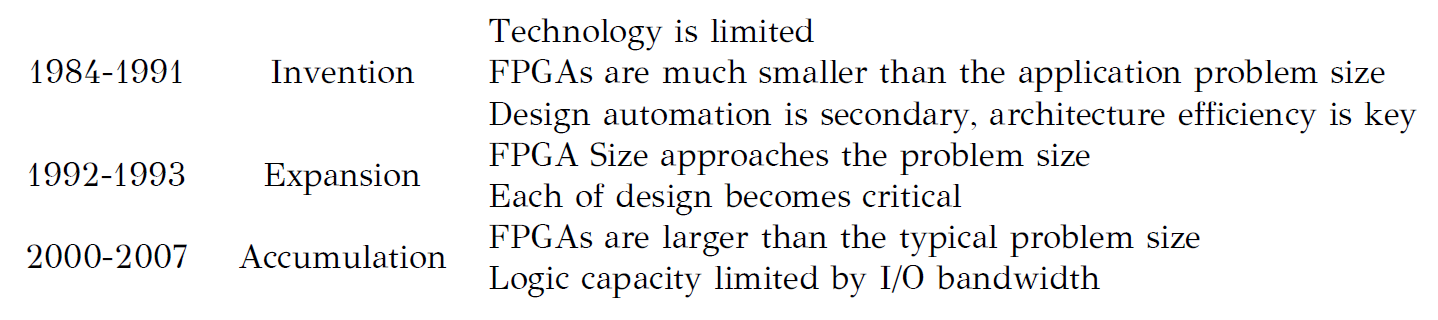
\includegraphics[width=0.95\textwidth]{images/eras}\\
  \caption{FPGA Eras}
\end{figure}

Παροδοσιακά, τα \gls{fpga}s ήταν αργά, είχαν μεγάλη κατανάλωση ισχύος και παρείχαν μικρότερη λειτουργικότητα από τα \gls{asic}s. Ωστόσο, στη σημερινή εποχή έχουν εξελιχθεί δραματικά και παρέχουν λύσεις που τα καθιστούν ιδανικότερη λύση. Μπορούν να επιτύχουν:
\begin{itemize}
	\item Χαμηλή κατανάλωση ισχύος
	\item Αυξημένη ταχύτητα
	\item Χαμηλό κόστος
	\item 'On-the-fly' διαμόρφωση \\
\end{itemize}

Η εξέλιξη αυτή δε θα μπορούσε να έχει επιτευχθεί χωρίς τη βοήθεια της ραγδαίας αύξησης του αριθμού των λογικών πυλών των \gls{fpga}s.
\begin{itemize}
	\item 1982: 8192 πύλες
	\item 1987: 9,000 πύλες
	\item 1992: 600,000 πύλες
	\item Early 2000s: Εκατομμύρια \\
\end{itemize}

Ιδιαίτερη μνεία πρέπει να γίνει στη νέα αρχιτεκτονική που αναπτύσσεται τα τελευταία χρόνια, τα \gls{soc} class \gls{fpga}s. Ένα \gls{soc} είναι ένα chip το οποίο περιλαμβάνει έναν ή περισσότερους πυρήνες -- μικροεπεξεργαστές και/ή DSP μαζί με μνήμη και διάφορα περιφερειακά. Με τη πάροδο του χρόνου οι δυνατότητες των \gls{fpga} έχουν παρουσιάσει δραματική αύξηση και ένα σύγχρονο \gls{fpga} μπορεί να περιλαμβάνει χιλιάδες αθροιστές, DSP slices κα. όμως το πρόβλημα που εμφανίζεται είναι ότι πλέον δεν αντανακλούν τις δυνατότητες και τη λειτουργικότητα των σύγχρονων προγραμματιζόμενων συσκευών. Για το λόγο αυτό δημιουργήθηκαν τα \gls{soc} class \gls{fpga}s τα οποία μπορούν να περιέχουν έναν η περισσότερους soft/hard πυρήνες ARM μαζί με περιφερειακά και μνήμη συνδυάζοντας κατ' αυτόν τον τρόπο την απόδοση και την εξοικονόμηση ενέργειας των \glspl{ip} με την ευελιξία του προγραμματισμού του επεξεργαστή ARM. Τα \gls{apsoc} όπως τα ονομάζει η Xilinx είναι ιδανικά για:
\hyphenation{pro-ces-sor}
\hyphenation{ban-dwidth}
\begin{itemize}
  \item Ελαχιστοποίηση κατανάλωσης, κόστους, μεγέθους πλακέτας ενσωματώνοντας διακριτούς μικροεπεξεργαστές και συναρτήσεις DSP σε ένα FPGA
  \item Βελτιστοποίηση της απόδοσης του συστήματος με τη βοήθεια μίας high-bandwidth διασύνδεσης μεταξύ του επεξεργαστή και του FPGA
  \item Βελτίωση της διαφορετικότητας του τελικού προϊόντος προσαρμόζοντας κατάλληλα τόσο το υλικό όσο και το λογισμικό
  \item Ανάπτυξη εφαρμογών συμβατών με την αρχιτεκτονική ARM με απαράμιλλο έλεγχο και παραγωγικότητα κάνοντας χρήση του FPGA-Adaptive debugging
\end{itemize}
\subsection{Εφαρμογές}

Τα FPGA μπορούν να επιλύσουν οποιοδήποτε πρόβλημα είναι δυνατόν να επιλυθεί υπολογιστικά. Η πρόταση αυτή έχει τεκμηριωθεί από το γεγονός ότι έχει επιτευχθεί ο σχεδιασμός ένος soft μικροεπεξεργαστή όπως για παράδειγμα ο Microblaze της Xilinx. Το πλεονέκτημα τους βρίσκεται στο ότι ορισμένες φορές είναι σημαντικά πιο γρήγοροι για συγκεκριμένες εφαρμογές λόγω της παραλληλίας και της βελτιστοποίησης που προσφέρουν. Ένα μεγάλο πλεονέκτημα των FPGA είναι ότι μπορούν να χρησιμοποιηθούν σαν επιταχυντές υλικού, όπου ο σχεδιαστής μπορεί να το χρησιμοποιήσει για να επιταχύνει \textbf{συγκεκριμένα} κομμάτια του αλγορίθμου και να μοιράσει μέρος του υπολογιστικού φόρτου με κάποιον μικροεπεξεργαστή γενικού σκοπού. Συνήθεις εφαρμογές των FPGA είναι στους τομείς που ακολουθούν:
\begin{itemize}
  \item Aerospace \& Defense
  \item Medical Electronics
  \item Audio
  \item Automotive
  \item Consumer Electronics
  \item Data Centers
  \item High Performance Computing
  \item Industrial κά. \\
\end{itemize}
\subsection{Σχεδιασμός υλικού \& Προγραμματισμός FPGA}

Για την περιγραφή της συμπεριφοράς ενός FPGA, ο σχεδιαστής παρέχει ένα πρόγραμμα γραμμένο σε κάποια γλώσσα περιγραφής υλικού (HDL) όπως για παράδειγμα σε VHDL ή Verilog. Μετά τη συγγραφή του κώδικα, με τη βοήθεια \gls{eda} εργαλείων ο χρήστης δημιουργεί ένα \gls{net} το οποίο μεταφέρει στο FPGA, συνήθως μέσω ιδιόκτητου λογισμικού της εκάστοτε εταιρίας. Ο σχεδιαστής τότε θα επιβεβαιώσει τη σωστή λειτουργία πραγματοποιώντας χρονική ανάλυση, προσομοίωση και άλλες διαφορτικές μεθοδολογίες. Όταν επιβεβαιωθεί τελικώς η σωστή λειτουργία, παράγεται το bitstream το οποίο χρησιμοποείται για τον (επανα)προγραμματισμό του FPGA. Το αρχείο αυτό μετφέρεται στο FPGA συνήθως μέσω της διεπαφής (JTAG).

Τα τελευταία χρόνια έχει αναπτυχθεί μία νέα τεχνική προγραμματισμού των FPGA για να αντικαταστήσει τον σχεδιασμό σε HDL που ονομάζεται \gls{hls}. Τα εργαλεία \gls{hls} αναλύουν μία υπάρχουσα εφαρμογή γραμμένη σε γλώσσα υψηλού επιπέδου - συνήθως C, C++, systemC και παράγουν την αντίστοιχη HDL. Το \gls{hls} έχει προοπτικές για να είναι το επόμενο σημαντικό βήμα για την ανάπτυξη προγραμμάτων σε FPGA.

Στην υποενότητα αυτή έγινε μια σύντομη αναφορά στον σχεδιασμό και προγραμματισμό των FPGA. Στο επόμενο κεφάλαιο θα εμβαθύνουμε περισσότερο στη χρήση σχεδιαστικών μεθοδολογιών υψηλού επιπέδου.

\section{Περιγραφή \& Στόχοι της εργασίας}

Όπως αναφέρθηκε στην προηγούμενη ενότητα ένας τρόπους ανάπτυξης σύνθετων εφαρμογών που απαιτούν μεγάλη επεξεργαστική ισχύ σε πραγματικό χρόνο με λογικό κόστος είναι η χρήση μονάδων FPGA με τον κατάλληλο προγραμματισμό τους σε ειδικές γλώσσες  (VHDL, Verilog). Σήμερα όμως, σε όλους τους κλάδους της βιομηχανίας, προκύπτουν ολοένα και περισσότερες τέτοιες εφαρμογές που μάλιστα πρέπει να υλοποιούνται σε ελάχιστο χρόνο κυρίως λόγω του ανταγωνισμού αλλά και των απαιτήσεων των χρηστών. Η ανάπτυξη αυτών των εφαρμογών σε FPGA απαιτεί απασχόληση μεγάλου πλήθους απολύτως εξειδικευμένου προσωπικού για μεγάλο χρονικό διάστημα μέχρι την υλοποίησή τους, γεγονός που προκάλεσε την ανάπτυξη της πλατφόρμας Vivado \gls{hls} και τον προγραμματισμό σε κάποια διαδεδομένη γλώσσα υψηλού επιπέδου.

Διαφαίνεται έτσι ότι η λύση με την υλοποίηση της εφαρμογής μέσω της πλατφόρμας Vivado \gls{hls} εμφανίζει πολλά πλεονεκτήματα  (μικρός χρόνος ανάπτυξης, χαμηλότερο κόστος κλπ). Αυτό σημαίνει ότι είναι απαραίτητη η όσο το δυνατόν μεγαλύτερη διάδοση και εξοικείωση των νέων μηχανικών στην όλη διαδικασία χρήσης της πλατφόρμας \gls{hls} αλλά και η ολοκλήρωση (integration) των παραγόμενων αποτελεσμάτων σε FPGA μέσω κατάλληλου υλικού και λογισμικού. Η παρούσα εργασία αυτόν ακριβώς το στόχο έχει. Να περιγράψει:
\begin{itemize}
\item{την ανάπτυξη και την end-to-end υλοποίηση μιας απαιτητικής εφαρμογής Υπολογιστικής Όρασης σε FPGA με τη χρήση της πλατφόρμας Vivado \gls{hls}}
\item{τη διαπίστωση και καταγραφή τυχόν προβλημάτων και δυσκολιών που έχουν προκύψει}
\item{τον έλεγχο των παραγόμενων αποτελεσμάτων και την υλοποίηση τεχνικών βελτίωσης της λειτουργίας του συστήματος}
\item{τα σημεία στα οποία η εργασία μπορεί να αναπτυχθεί ή να βελτιωθεί μελλοντικά}
\end{itemize}
\section{Διάρθρωση της διπλωματικής}
\noindent
Το κείμενο της διπλωματικής είναι διαχωρισμένο σε 8 κεφάλαια. Αρχικά, γίνεται μια εισαγωγή στα FPGA, στη συνέχεια παρουσιάζεται η υπολογιστική όραση και στο τέλος γίνεται αναλυτική περιγραφή της υλοποίησης και παρουσίαση των αποτελεσμάτων και συμπερασμάτων. \\

\begin{itemize}[label={},leftmargin=*]
\item \textbf{Κεφάλαιο 1}

Γίνεται μια εισαγωγή στα FPGA και στην τεχνολογία τους, στις πολλαπλές εφαρμογές τους καθώς και στον τρόπο προγραμματισμού τους. Παρουσιάζονται επίσης οι στόχοι της διπλωματικής εργασίας. \\

\item \textbf{Κεφάλαιο 2}

Παρουσιάζεται η βασική αρχιτεκτονική των σύγχρονων FPGA καθώς και της πλατφόρμας που θα χρησιμοποιηθεί κατα τη διάρκεια της εργασίας. Αναλύεται η ανάπτυξη λογισμικού για την περιγραφή του υλικού με έμφαση στη High Level Synthesis.\\

\item \textbf{Κεφάλαιο 3}

Γίνεται μία εις βάθος ανάλυση της υπολογιστικής όρασης και παρουσιάζονται οι εφαρμογές της, η ροή ανάπτυξης εφαρμογών και η σχέση της με τα FPGA.\\

\item \textbf{Κεφάλαιο 4}

Αρχικά, γίνεται μία εισαγωγή στην αναγνώριση ακμών και έπειται αναλύεται η μέθοδος αναγνώρισης ακμών με τη μέθοδο του Canny. Παρουσιάζονται όλα τα απαραίτητα βήματα και προσεγγίσεις.

\item \textbf{Κεφάλαιο 5}

Παρουσιάζεται η πλήρης υλοποίηση του ενσωματωμένου συστήματος. Γίνεται περιγραφή της ροής στο \gls{hls}, ο σχεδιασμός του συστήματος με τα απαιτούμενα περιφερειακά και τέλος αναλύεται η εφαρμογή του επεξεργαστή και η εκτέλεση του προγράμματος. \\

\item \textbf{Κεφάλαιο 6}

Παρατίθενται διάφορες βελτιστοποιήσεις που έγιναν κατά την ανάπτυξη του αλγορίθμου και τα αποτέλεσματα της υλοποίησης. \\

\item \textbf{Κεφάλαιο 7}

Στο κεφάλαιο αυτό αναλύουμε τα συμπεράσματα που προέκυψαν από την υλοποίηση και δίνονται απαντήσεις σε ερωτήματα που προέκυψαν κατά τη διάρκεια της εργασίας. Γίνεται επίσης αναφορά στις διάφορες δυσκολίες που εμφανίστηκαν. Τέλος, γίνεται λόγος και στις μελλοντικές εργασίες που μπορούν να πραγματοποιηθούν.
\end{itemize}

\section{Behind the project}

Όπως αναφέρθηκε και στην προηγούμενη υποενότητα, το \gls{hls} είναι μια συνεχώς αναπτυσσόμενη τεχνολογία που μπορεί να αντικαταστήσει τον παραδοσιακό τρόπου σχεδιασμού και προγραμματισμού των FPGA. Η ευκαιρία να μελετήσουμε σε βάθος και να βγάλουμε συμπεράσματα για την τεχνολογία αυτή αποτέλεσε και το βασικότερο κίνητρο για την πραγματοποίηση της συγκεκριμένης διπλωματικής εργασίας.

Ελπίζουμε ότι η εργασία αυτή θα αποτελέσει κίνητρο και το πρώτο σκαλί για λεπτομερέστερη μελέτη της διαδικασίας προγραμματισμού των FPGAs μέσω της γλώσσας υψηλού επιπέδου \gls{hls} ώστε η ανάπτυξη σύνθετων ηλεκτρονικών μονάδων να γίνει απλούστερη και οικονομικότερη.